\documentclass[aspectratio=169]{beamer}
%
% Choose how your presentation looks.
%
% For more themes, color themes and font themes, see:
% http://deic.uab.es/~iblanes/beamer_gallery/index_by_theme.html
%
\mode<presentation>
%{https://writelatex.s3.amazonaws.com/vpzdvfpgmtcs/page/20577db5fb5206cebb645db53626924bd7e5686f.jpeg}
  \usetheme{Frankfurt}      % or try Darmstadt, Madrid, Warsaw, ...
  \usecolortheme{beaver} % or try albatross, beaver, crane, ...
  \usefonttheme{default}  % or try serif, structurebold, ...
  \setbeamertemplate{navigation symbols}{}
  \setbeamertemplate{caption}[numbered]{}
\setbeamertemplate{footline}[frame number]

\usepackage[english]{babel}
\usepackage[utf8x]{inputenc}
\usepackage{hyperref}
\usepackage{graphicx}
\usepackage{moreverb}

\title[GetL_Presentation]{Grammaires et Langages : Présentation}
\author{Equipe Minizza - H4111}
\institute{INSA de Lyon}
\date{Mardi 1 Mars}

\begin{document}

\begin{frame}
\titlepage
\end{frame}

% Plan proposé :
%
% 1. 


\section{Structures de données}
\subsection{Diagramme de classes}
\begin{frame}{Diagramme de classes}
\begin{center}
 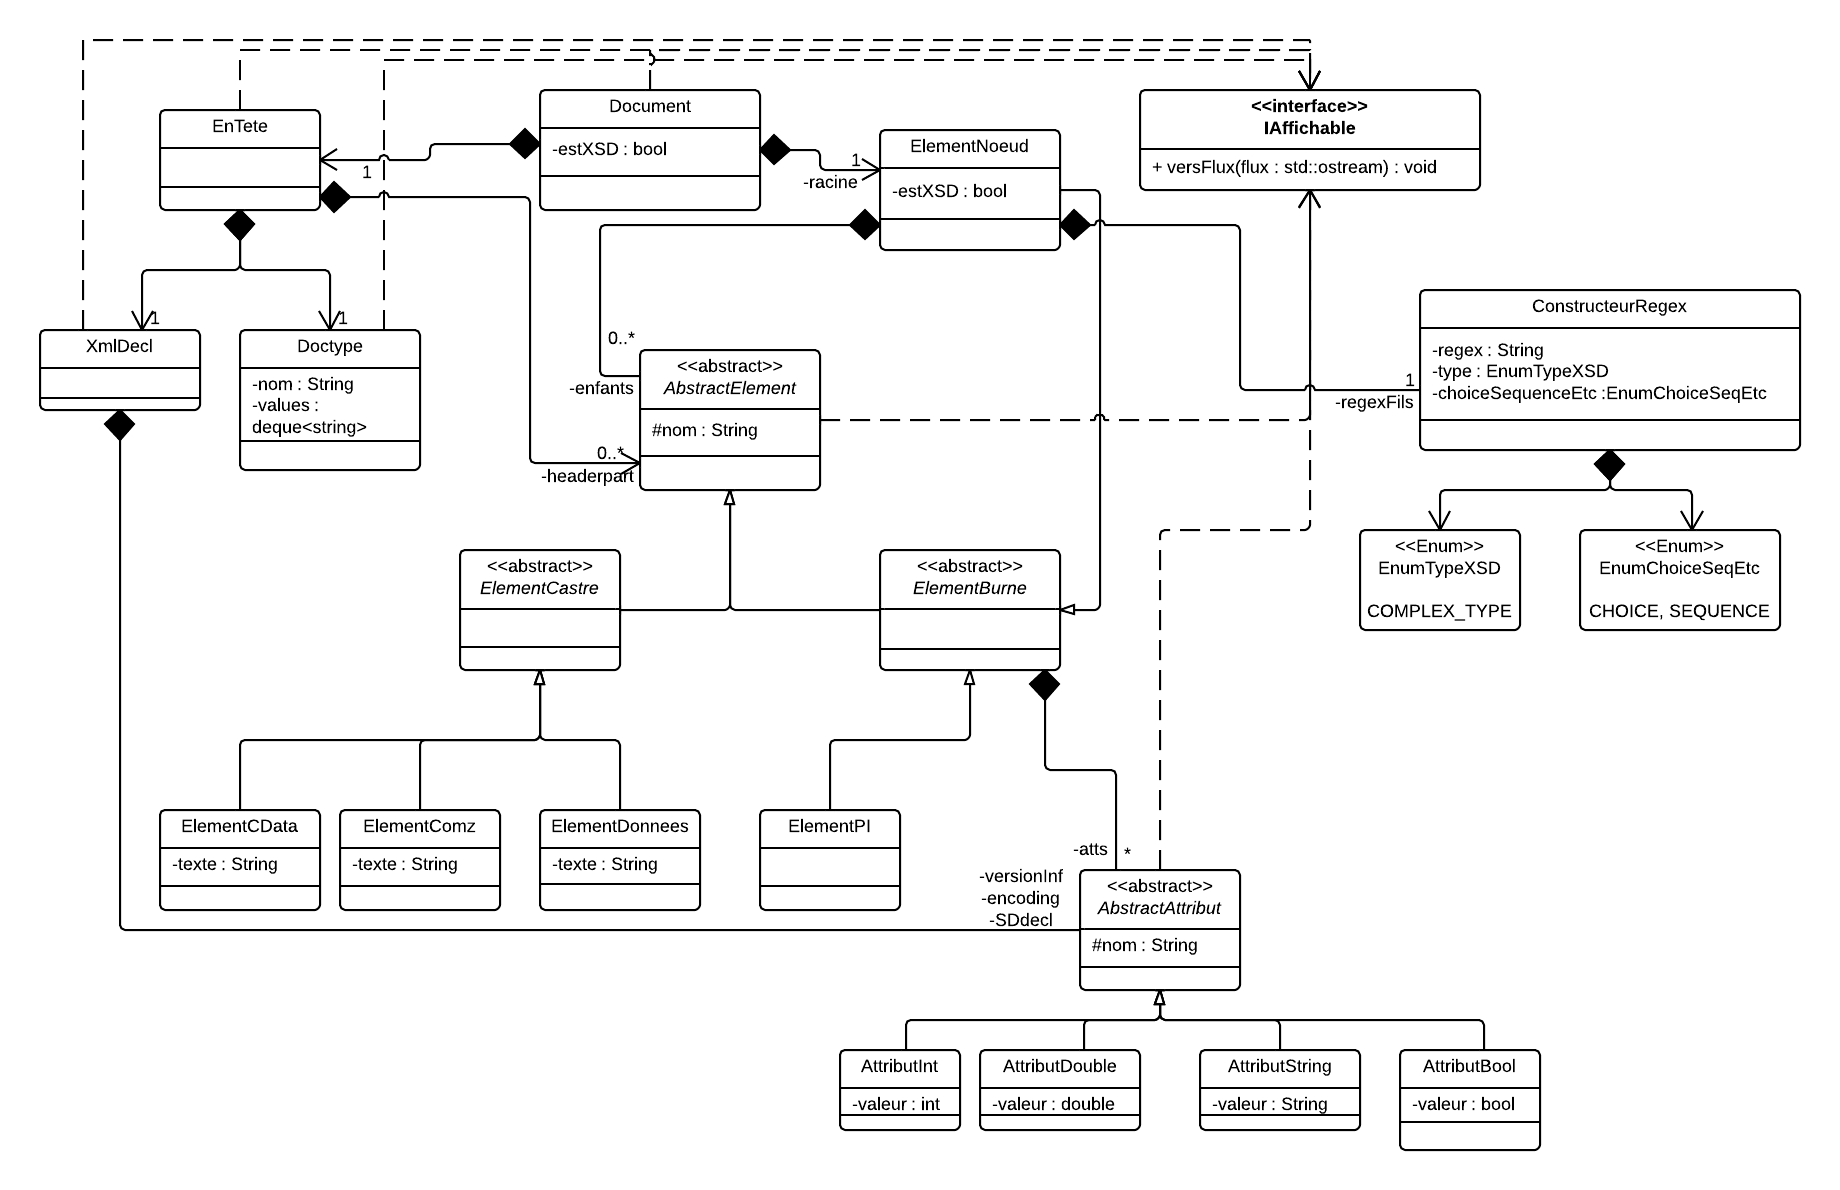
\includegraphics[scale=0.17]{diagdcla}
\end{center}
\end{frame}

\subsection{Diagramme de classes}
\begin{frame}{Diagramme de classes}
\begin{center}
  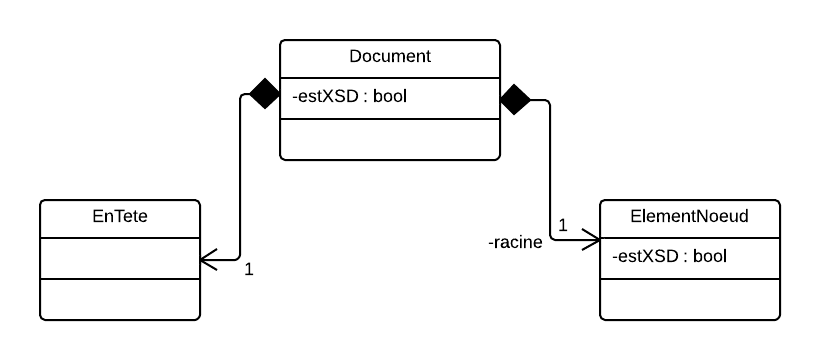
\includegraphics[scale=0.3]{ddc_doc}
\end{center}
\end{frame}

\subsection{Diagramme de classes}
\begin{frame}{Diagramme de classes}
\begin{center}
 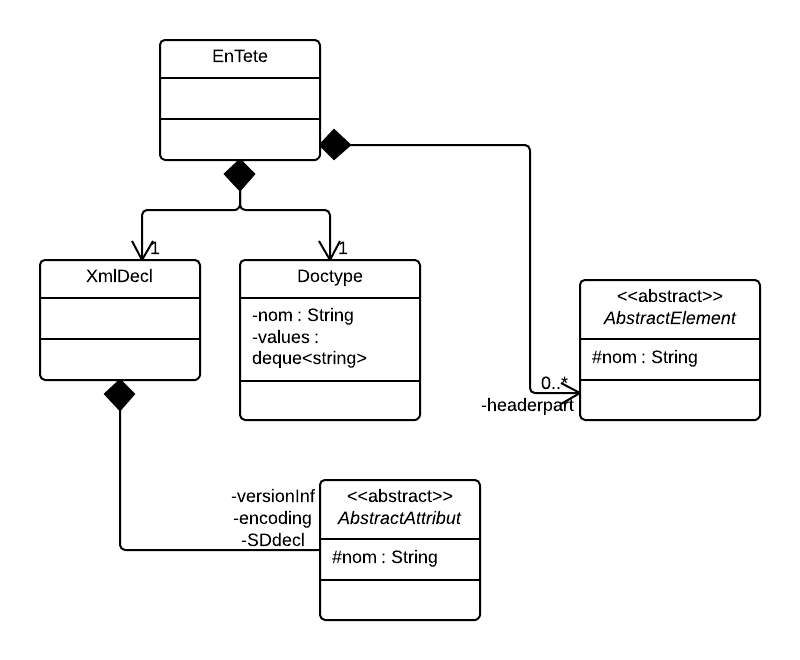
\includegraphics[scale=0.3]{ddc_ent}
\end{center}
\end{frame}

\subsection{Diagramme de classes}
\begin{frame}{Diagramme de classes}
\begin{center}
  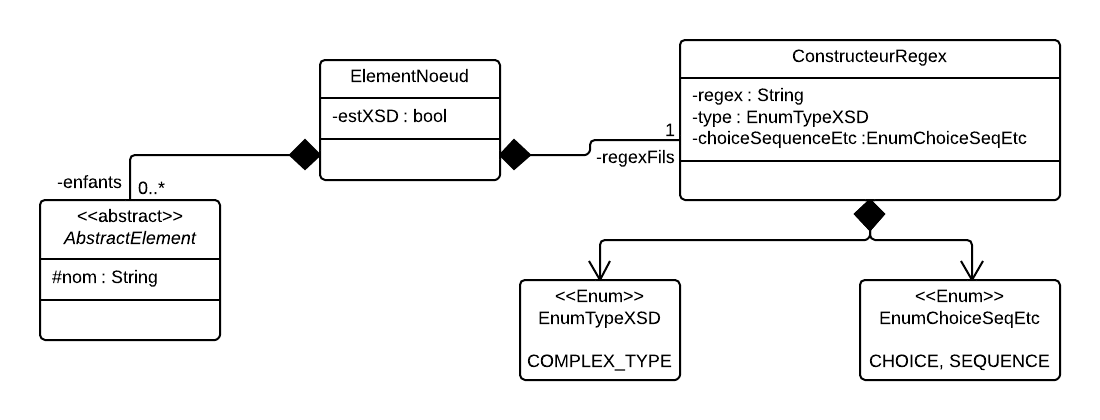
\includegraphics[scale=0.3]{ddc_noeud}
\end{center}
\end{frame}

\subsection{Diagramme de classes}
\begin{frame}{Diagramme de classes}
\begin{center}
  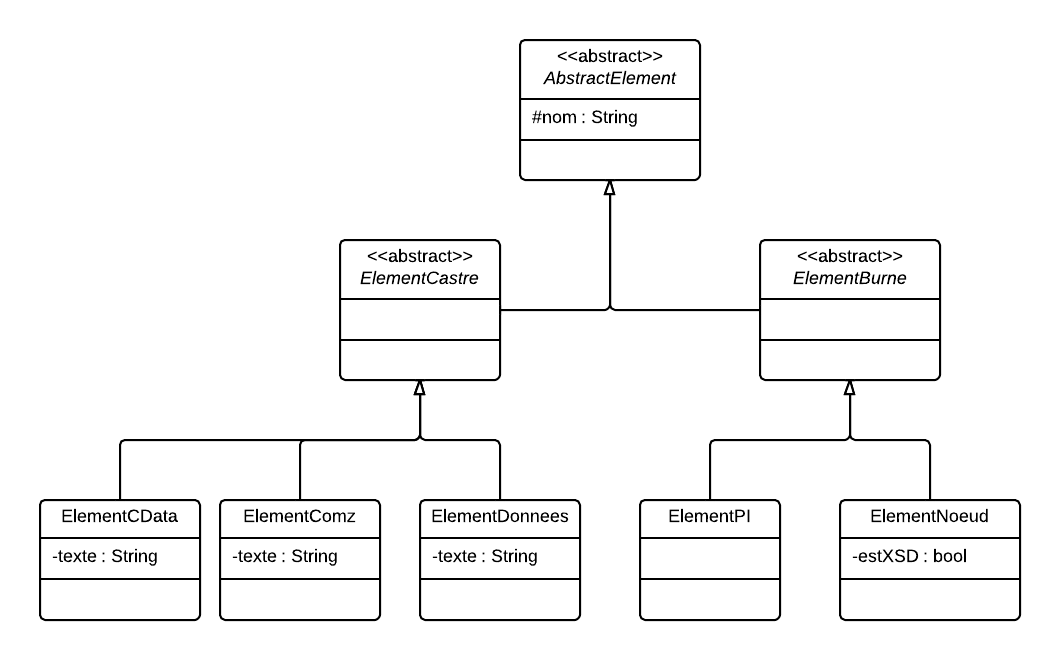
\includegraphics[scale=0.3]{ddc_abs_elmt}
\end{center}
\end{frame}

\subsection{Diagramme de classes}
\begin{frame}{Diagramme de classes}
\begin{center}
  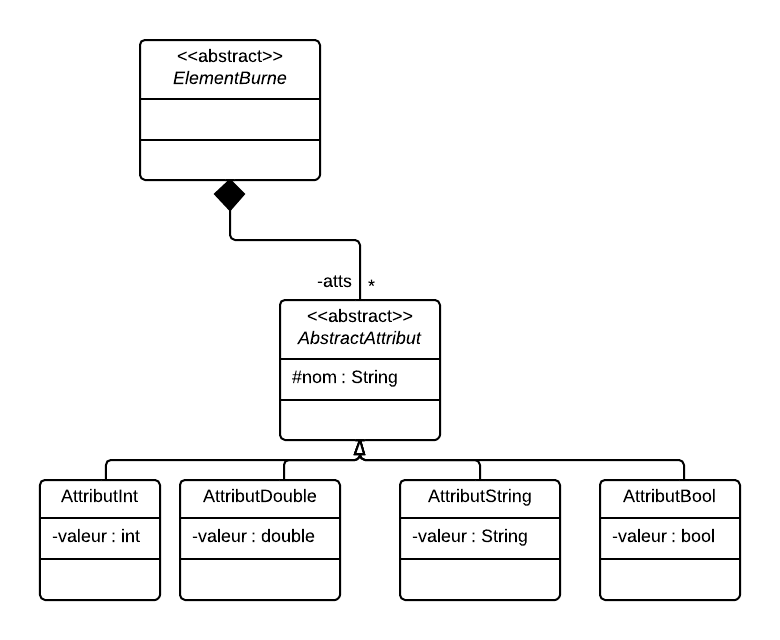
\includegraphics[scale=0.3]{ddc_elmt_burne}
\end{center}
\end{frame}

\subsection{Diagramme de classes}
\begin{frame}{Diagramme de classes}
\begin{center}
  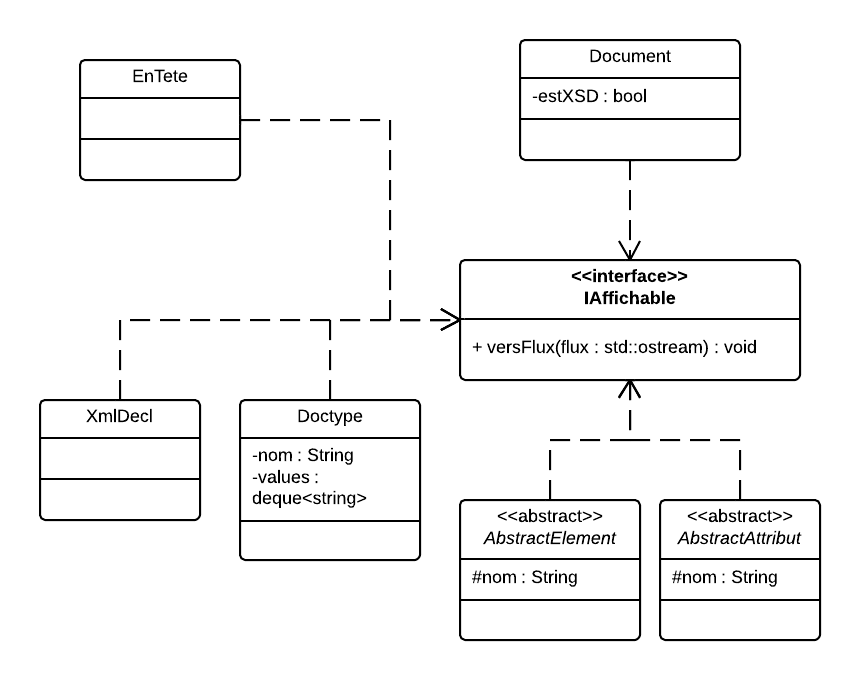
\includegraphics[scale=0.3]{ddc_iaff}
\end{center}
\end{frame}


\section{Algorithme de  validation}
\subsection{Algorithme de  validation}
\begin{frame}{Algorithme de validation}
 
\end{frame}

\section{Algorithme de transformation}
\subsection{Algorithme de transformation}
\begin{frame}{Algorithme de transformation}
 
\end{frame}

\subsection{Algorithme de transformation}
\begin{frame}[fragile]{Algorithme de transformation - Fonctions Utiles }
 Fonctions de AbstractElement et redéfinies dans ElementDonnees
 \scriptsize
 \begin{verbatim}
  String obtenirDonnees()
Elle retourne "" pour abstractelement et noeud.texte pour elementdonnees

APPEL INITIAL DE LA FONCTION
racineXSL = documentXSL.racine.enfants.trouver(xsl:template match="/")
racineXML = documentXML.racine
sortie = racineXSL.TransformationXSL(racineXML, "")
 \end{verbatim}
\normalsize
\end{frame}

\subsection{Algorithme de transformation}
\begin{frame}[fragile]{Algorithme de transformation}
Fonction de AbstractElement
\scriptsize
\begin{verbatim}
 String TransformationXSL(noeudXML, sortie)
    retourner sortie
\end{verbatim}
\end{frame}

\subsection{Algorithme de transformation}
\begin{frame}[fragile]{Algorithme de transformation}
 Fonctions de ElementDonnees
 \scriptsize
 \begin{verbatim}
  String TransformationXSL(noeudXML, sortie)
    retourner sortie += noeudCourantXSL.texte
 \end{verbatim}
 \normalsize
\end{frame}

\subsection{Algorithme de transformation}
\begin{frame}{Algorithme de transformation}
 Fonctions de ElementNoeud\\
 \scriptsize
String TransformationXSL(noeudXML, sortie)\\
\begin{enumerate}
 \item si noeudXSLCourant est value-of
 \item si noeudXSLCourant est fore-each
 \item si noeudXSLCourant est rien
 \item si noeudXSLCourant est apply-template avec attribut
 \item si noeudXSLCourant est apply-template sans attribut
 \item si noeudXSLCourant est template
\end{enumerate}
retour sortie
\normalsize
\end{frame}

\subsection{Algorithme de transformation}
\begin{frame}[fragile]{Algorithme de transformation}
1) value-of
\scriptsize
\begin{verbatim}
si select est "." alors
    pour filsXML de noeudXML faire
        sortie += filsXML.obtenirDonnees()
sinon
    enfantsXML = tous les filsXML de noeudXML tels que filsXML.nom = select
    pour enfantXML de enfantsXML faire
        sortie += enfantXML.obtenirDonnees()
\end{verbatim}
\normalsize
\end{frame}

\subsection{Algorithme de transformation}
\begin{frame}[fragile]{Algorithme de transformation}
 2) fore-each
 \scriptsize
 \begin{verbatim}
  enfantsXML = tous les filsXML de noeudXML tels que filsXML.nom = select
pour enfantXML de enfantsXML faire
    sortie += noeud\_foreach.TransformationXSL(enfantXML, sortie)
 \end{verbatim}
\normalsize
\end{frame}

\subsection{Algorithme de transformation}
\begin{frame}[fragile]{Algorithme de transformation}
 3) Rien (pas de balises xsl spéciale)
 \scriptsize
 \begin{verbatim}
  sortie += "<" + noeudXSL.nom
pour attribut de noeudXSL.attributs faire
    sortie += " " + attribut.nom + "=" + attribut.valeur
sortie += ">"
pour filsXSL de noeudXSL faire
    sortie += filsXSL.TransformationXSL(noeudXML, sortie)    
sortie += "</" + noeudXSL.nom + ">"
 \end{verbatim}
\normalsize
\end{frame}

\subsection{Algorithme de transformation}
\begin{frame}[fragile]{Algorithme de transformation}
 4) apply-templates select="something"
 \scriptsize
 \begin{verbatim}
  templateXSL = noeudXSL template tel que noeudXSL.match = select
enfantsXML = tous les filsXML de noeudXML tels que filsXML.nom = select
pour enfantXML de enfantsXML faire
    sortie += templateXSL.TransformationXSL(enfantXML, sortie)
 \end{verbatim}
\normalsize
\end{frame}

\subsection{Algorithme de transformation}
\begin{frame}[fragile]{Algorithme de transformation}
 5) apply-templates sans attribut
 \scriptsize
 \begin{verbatim}
  enfantsXML = tous les filsXML de noeudXML
pour enfantXML de enfantsXML faire
    templateXSL = noeudXSL tel que noeudXSL.match = enfantXML.nom
    sortie += templateXSL.TransformationXSL(enfantXML, sortie)
 \end{verbatim}
\normalsize
\end{frame}

\subsection{Algorithme de transformation}
\begin{frame}[fragile]{Algorithme de transformation}
 6) template match="something"
 \scriptsize
 \begin{verbatim}
  pour filsXSL de noeudXSL faire
    sortie += filsXSL.TransformationXSL(noeudXML, sortie)
 \end{verbatim}
\normalsize
\end{frame}

\section{Bilan du projet}
\subsection{Bilan quatitatif}
\begin{frame}{Bilan quantitatif}
\begin{center}
 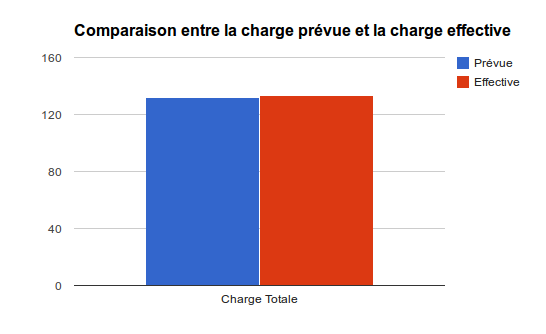
\includegraphics[scale=0.5]{chargetot}
\end{center}
\end{frame}

\subsection{Bilan quatitatif}
\begin{frame}{Bilan quantitatif}
\begin{center}
 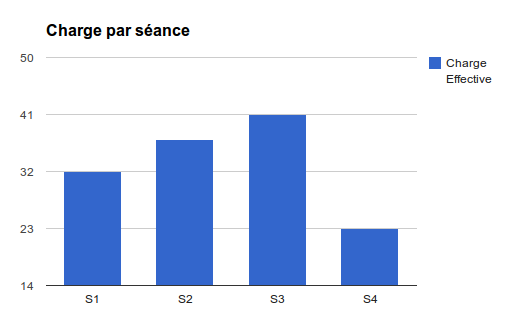
\includegraphics[scale=0.5]{chargeseance}
\end{center} 
\end{frame}

\subsection{Bilan quatitatif}
\begin{frame}{Bilan quantitatif}
 \begin{center}
 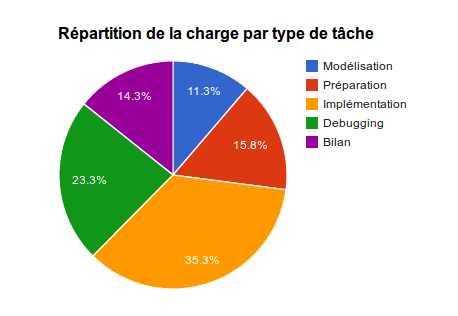
\includegraphics[scale=0.5]{chargetype}
\end{center}
\end{frame}

\subsection{Bilan qualitatif}
\begin{frame}{Bilan qualitatif}
Montées en compétence :
\begin{itemize}
 \item Modélisation pas évidente
 \item Développer la syntaxe
 \item Retoucher au C++
 \item Implémentation difficile
 \item Analyse des langages XML, XSD, XSL
\end{itemize}
\end{frame}

\subsection{Bilan qualitatif}
\begin{frame}{Bilan qualitatif}
Ressenti vis à vis du projet :
 \begin{itemize}
  \item Framework de test génial, très agréable
  \item Aucun souci avec ce qui nous a été donné
  \item Un projet bien dimensionné
  \item Un projet intéressant
 \end{itemize}
\end{frame}



\end{document}